Using section formula,
\begin{align}
\vec{R}_k=\frac{\vec{B}+k\vec{A}}{1+k}
\end{align}
See 
\tabref{tab:10/7/2/9}
and 
\figref{fig:chapters/10/7/2/9/Fig}
\begin{table}[!ht]
\centering
\caption{}
\label{tab:10/7/2/9}
\begin{tabular}{|c|c|}
\hline
	$k$ & $\vec{R}_k$ \\
\hline
3 & 
\myvec{
-1\\
\\
\frac{7}{2}
}\\
\hline
1 & \myvec{
0\\
5
}
\\
\hline
	$\frac{1}{3}$ &\myvec{
1
\\
\frac{13}{2}
}
 \\
\hline
\end{tabular}
\end{table}
\begin{figure}[!h]
\begin{center}
   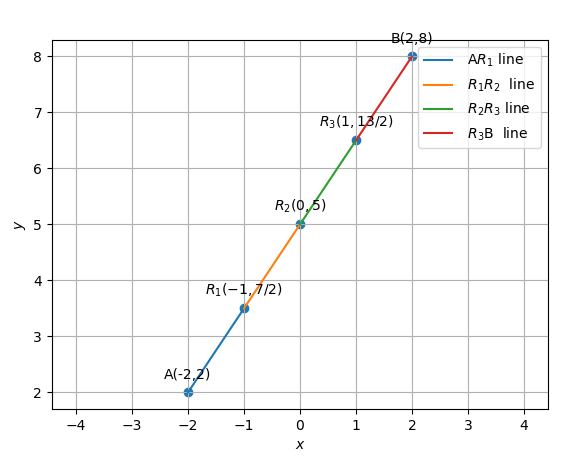
\includegraphics[width=\columnwidth]{chapters/10/7/2/9/figs/10.7.2.9.png}
\end{center}
\caption{}
\label{fig:chapters/10/7/2/9/Fig}
\end{figure}

